\documentclass[aps,prx,twocolumn,superscriptaddress,nofootinbib]{revtex4-2}
\usepackage{amsmath,amssymb,bm}
\usepackage{graphicx}
\usepackage{hyperref}

% Auto-generated by generate_rep5_softmwpm_bt2t004_paper_assets.py -- DO NOT EDIT BY HAND
\newcommand{\rfsPaperId}{\texttt{OSIRIS-REP5-SOFTMWPM-BT2T004-2026}}
\newcommand{\rfsBackend}{\texttt{ibm\_fez}}
\newcommand{\rfsHeronQubits}{156}
\newcommand{\rfsHwTier}{\texttt{HARDWARE\_ATTESTED}}
\newcommand{\rfsSimTier}{\texttt{SIMULATED}}
\newcommand{\rfsProxyTier}{\texttt{PROXY}}
\newcommand{\rfsSimJobId}{\texttt{null}}
\newcommand{\rfsSimQpuSec}{0}
\newcommand{\rfsCapsuleSha}{\texttt{e5deeb52f80b19d8...}}

% Manifest 1: OSIRIS-QEC-REP5-FEZ
\newcommand{\rfsRepFiveJobId}{\texttt{dc3bmlinj2vs73di19s0}}
\newcommand{\rfsRepFiveQpuSec}{12}
\newcommand{\rfsRepFiveTotalPubs}{72}
\newcommand{\rfsRepFiveShotsPerPub}{512}
\newcommand{\rfsRepFiveTotalShots}{36,864}
\newcommand{\rfsRepFiveShotsPerCell}{2,048}
\newcommand{\rfsRepFiveBlocks}{2}
\newcommand{\rfsRepFivePubsPerBlock}{36}
\newcommand{\rfsRepFiveChain}{\texttt{[120, 121, 122, 123, 136, 143, 142, 141, 140]}}
\newcommand{\rfsRepFiveDataChain}{\texttt{[120, 122, 136, 142, 140]}}
\newcommand{\rfsRepFiveAncChain}{\texttt{[121, 123, 143, 141]}}
\newcommand{\rfsRepThreeSubChain}{\texttt{[122, 123, 136, 143, 142]}}
\newcommand{\rfsRepFiveStagedCommit}{\texttt{82cfd46a}}
\newcommand{\rfsRepFiveWriteAheadHours}{3.39}
\newcommand{\rfsRepFiveQuotaBefore}{38.0}
\newcommand{\rfsRepFiveQuotaAfter}{26.0}
\newcommand{\rfsRepFiveRoundDt}{904}
\newcommand{\rfsRepFiveRoundUs}{3.616}
\newcommand{\rfsRepFiveRThreeUs}{10.848}
\newcommand{\rfsRepFiveRFiveUs}{18.080}
\newcommand{\rfsRepFiveQpyShaFull}{\texttt{da8061639e8eaa7e708f506095c590f69dc39ec5573f67edebadbb6f9416aee1}}
\newcommand{\rfsRepFiveQpyShaPrefix}{\texttt{da8061639e8eaa7e...}}
\newcommand{\rfsRepFiveRawGzShaFull}{\texttt{d73bd9c153d2feddc7e403455b6b725630106ee3b09d8d4f103bdb83fcadea56}}
\newcommand{\rfsRepFiveRawGzShaPrefix}{\texttt{d73bd9c153d2fedd...}}
\newcommand{\rfsRepFivePreregShaPrefix}{\texttt{18af4ae9aa2e0560...}}
\newcommand{\rfsRepFiveResultsShaPrefix}{\texttt{9e6ce1adbce6b1d0...}}
\newcommand{\rfsRepFiveRoCalFid}{0.947754}
\newcommand{\rfsRepFiveRoCalFidPct}{94.78\%}
\newcommand{\rfsRepFiveRoErrQOneTwoZero}{0.019694}
\newcommand{\rfsRepFiveRoErrQOneTwoTwo}{0.003255}
\newcommand{\rfsRepFiveRoErrQOneThreeSix}{0.012695}
\newcommand{\rfsRepFiveRoErrQOneFourZero}{0.012044}
\newcommand{\rfsRepFiveRoErrQOneFourTwo}{0.006673}
\newcommand{\rfsRepFiveCalRoMean}{0.01000}
\newcommand{\rfsRepFiveCalCzSum}{0.01832}
\newcommand{\rfsRepFiveArmOneROne}{0.023438}
\newcommand{\rfsRepFiveArmOneRThree}{0.039062}
\newcommand{\rfsRepFiveArmOneRFive}{0.065430}
\newcommand{\rfsRepFiveArmTwoDThreeROne}{0.001953}
\newcommand{\rfsRepFiveArmTwoDThreeRThree}{0.011719}
\newcommand{\rfsRepFiveArmTwoDThreeRFive}{0.020020}
\newcommand{\rfsRepFiveArmTwoDFiveROne}{0.000977}
\newcommand{\rfsRepFiveArmTwoDFiveRThree}{0.005859}
\newcommand{\rfsRepFiveArmTwoDFiveRFive}{0.017090}
\newcommand{\rfsRepFiveArmFourDThreeROne}{0.000977}
\newcommand{\rfsRepFiveArmFourDThreeRThree}{0.008301}
\newcommand{\rfsRepFiveArmFourDThreeRFive}{0.012695}
\newcommand{\rfsRepFiveArmFourDFiveROne}{0.000488}
\newcommand{\rfsRepFiveArmFourDFiveRThree}{0.002930}
\newcommand{\rfsRepFiveArmFourDFiveRFive}{0.008301}
\newcommand{\rfsRepFiveLamROne}{2.0000}
\newcommand{\rfsRepFiveLamRThree}{2.8333}
\newcommand{\rfsRepFiveLamRFive}{1.5294}
\newcommand{\rfsRepFiveLamNoCorrROne}{2.0000}
\newcommand{\rfsRepFiveLamNoCorrRThree}{2.0000}
\newcommand{\rfsRepFiveLamNoCorrRFive}{1.1714}
\newcommand{\rfsRepFiveMeanLam}{2.1209}
\newcommand{\rfsRepFivePeakLam}{2.8333}
\newcommand{\rfsRepFiveROneGainVsBare}{48.0\times}
\newcommand{\rfsRepFiveRThreeGainVsBare}{13.33\times}
\newcommand{\rfsRepFiveRFiveGainVsBare}{7.88\times}
\newcommand{\rfsRepFiveRFiveGainVsNoCorr}{2.06\times}
\newcommand{\rfsRepFiveBlkDThreeROneA}{0.000977}
\newcommand{\rfsRepFiveBlkDThreeROneB}{0.000977}
\newcommand{\rfsRepFiveBlkDFiveROneA}{0.000977}
\newcommand{\rfsRepFiveBlkDFiveROneB}{0.000000}
\newcommand{\rfsRepFiveBlkDThreeRThreeA}{0.005859}
\newcommand{\rfsRepFiveBlkDThreeRThreeB}{0.010742}
\newcommand{\rfsRepFiveBlkDFiveRThreeA}{0.002930}
\newcommand{\rfsRepFiveBlkDFiveRThreeB}{0.002930}
\newcommand{\rfsRepFiveBlkDThreeRFiveA}{0.010742}
\newcommand{\rfsRepFiveBlkDThreeRFiveB}{0.014648}
\newcommand{\rfsRepFiveBlkDFiveRFiveA}{0.007812}
\newcommand{\rfsRepFiveBlkDFiveRFiveB}{0.008789}
\newcommand{\rfsRepFiveSlopeArmOne}{0.010498}
\newcommand{\rfsRepFiveSlopeArmTwoDThree}{0.004517}
\newcommand{\rfsRepFiveSlopeArmTwoDFive}{0.004028}
\newcommand{\rfsRepFiveSlopeArmFourDThree}{0.002929}
\newcommand{\rfsRepFiveSlopeArmFourDThreeRounded}{0.002930}
\newcommand{\rfsRepFiveSlopeArmFourDFive}{0.001953}
\newcommand{\rfsRepFiveSlopeRatio}{1.4998}
\newcommand{\rfsRepFiveSlopeRatioRounded}{1.5000}
\newcommand{\rfsRepFiveArmThreePostselZero}{0.000000}
\newcommand{\rfsRepFiveAccDThreeROnePct}{90.7\%}
\newcommand{\rfsRepFiveAccDThreeRThreePct}{79.2\%}
\newcommand{\rfsRepFiveAccDThreeRFivePct}{70.3\%}
\newcommand{\rfsRepFiveAccDFiveROnePct}{79.3\%}
\newcommand{\rfsRepFiveAccDFiveRThreePct}{60.6\%}
\newcommand{\rfsRepFiveAccDFiveRFivePct}{48.4\%}
\newcommand{\rfsRepFiveStreakRThreeA}{4.6282}
\newcommand{\rfsRepFiveStreakRThreeB}{5.3589}
\newcommand{\rfsRepFiveStreakRThreeC}{7.7350}
\newcommand{\rfsRepFiveStreakRThreeD}{5.9285}
\newcommand{\rfsRepFiveStreakRFiveA}{4.2123}
\newcommand{\rfsRepFiveStreakRFiveB}{5.2718}
\newcommand{\rfsRepFiveStreakRFiveC}{6.6705}
\newcommand{\rfsRepFiveStreakRFiveD}{4.8683}

% Manifest 2: OSIRIS-QEC-SOFTMWPM
\newcommand{\rfsSoftRepShaPrefix}{\texttt{86c6f35b813f6b21...}}
\newcommand{\rfsSoftHotFracPct}{25\%}
\newcommand{\rfsSoftPRoCal}{0.0083}
\newcommand{\rfsSoftPRoHotA}{0.032}
\newcommand{\rfsSoftPRoHotB}{0.060}
\newcommand{\rfsSoftPRoHotC}{0.100}
\newcommand{\rfsSoftPRoHotAPct}{3.2\%}
\newcommand{\rfsSoftPRoHotBPct}{6.0\%}
\newcommand{\rfsSoftPRoHotCPct}{10.0\%}
\newcommand{\rfsSoftBlossomSyndromes}{600}
\newcommand{\rfsSoftSinkholeTriangles}{38}
\newcommand{\rfsSoftTimeFloor}{0.05}
\newcommand{\rfsSoftGamma}{2.4}
\newcommand{\rfsSoftSurfStaleLamA}{1.269}
\newcommand{\rfsSoftSurfStaleLamACiLo}{1.00}
\newcommand{\rfsSoftSurfStaleLamACiHi}{1.62}
\newcommand{\rfsSoftSurfStaleLamB}{1.273}
\newcommand{\rfsSoftSurfStaleLamC}{1.235}
\newcommand{\rfsSoftSurfPriorLamA}{1.989}
\newcommand{\rfsSoftSurfPriorLamB}{2.019}
\newcommand{\rfsSoftSurfPriorLamC}{1.800}
\newcommand{\rfsSoftSurfSoftLamA}{3.537}
\newcommand{\rfsSoftSurfSoftLamACiLo}{2.57}
\newcommand{\rfsSoftSurfSoftLamACiHi}{5.21}
\newcommand{\rfsSoftSurfSoftLamB}{3.633}
\newcommand{\rfsSoftSurfSoftLamBCiLo}{2.78}
\newcommand{\rfsSoftSurfSoftLamBCiHi}{5.18}
\newcommand{\rfsSoftSurfSoftLamC}{3.334}
\newcommand{\rfsSoftSurfSoftLamCCiLo}{2.62}
\newcommand{\rfsSoftSurfSoftLamCCiHi}{4.45}
\newcommand{\rfsSoftSurfSoftLamFiveSevenMin}{3.50}
\newcommand{\rfsSoftSurfSoftLamFiveSevenMax}{4.36}
\newcommand{\rfsSoftRepStaleLamA}{1.180}
\newcommand{\rfsSoftRepStaleLamB}{0.817}
\newcommand{\rfsSoftRepStaleLamC}{0.848}
\newcommand{\rfsSoftRepSoftLamA}{4.061}
\newcommand{\rfsSoftRepSoftLamB}{3.252}
\newcommand{\rfsSoftRepSoftLamC}{4.296}
\newcommand{\rfsSoftFezRepThreeJobId}{\texttt{dc35d4inj2vs73dhmsog}}
\newcommand{\rfsSoftFezTotalShots}{49,152}
\newcommand{\rfsSoftFezArmFourShots}{9,216}
\newcommand{\rfsSoftFezChain}{\texttt{[58, 71, 70, 69, 78]}}
\newcommand{\rfsSoftFezROneUnif}{0.012370}
\newcommand{\rfsSoftFezROneSoft}{0.003255}
\newcommand{\rfsSoftFezROneRedPct}{73.68\%}
\newcommand{\rfsSoftFezRThreeUnif}{0.054036}
\newcommand{\rfsSoftFezRThreePrior}{0.039062}
\newcommand{\rfsSoftFezRThreeSoft}{0.011719}
\newcommand{\rfsSoftFezRThreeRedPct}{78.31\%}
\newcommand{\rfsSoftFezRThreeBlockT}{9.0138}
\newcommand{\rfsSoftFezRThreeBlockP}{0.006043}
\newcommand{\rfsSoftFezRThreePooledT}{12.60}
\newcommand{\rfsSoftFezRThreePooledP}{0.0031}
\newcommand{\rfsSoftFezRFiveUnif}{0.087240}
\newcommand{\rfsSoftFezRFivePrior}{0.063802}
\newcommand{\rfsSoftFezRFiveSoft}{0.022786}
\newcommand{\rfsSoftFezRFiveRedPct}{73.88\%}
\newcommand{\rfsSoftFezRFiveBlockT}{13.3792}
\newcommand{\rfsSoftFezRFiveBlockP}{0.002770}
\newcommand{\rfsSoftFezRFivePooledT}{13.91}
\newcommand{\rfsSoftFezRFivePooledP}{0.0026}
\newcommand{\rfsSoftFezSlopeUnif}{0.018717}
\newcommand{\rfsSoftFezSlopePrior}{0.012858}
\newcommand{\rfsSoftFezSlopeSoft}{0.004883}
\newcommand{\rfsSoftFezSlopeRedPct}{73.91\%}
\newcommand{\rfsSoftFezSlopeFactor}{3.83\times}
\newcommand{\rfsSoftFezAsymQFiveEight}{40.0\times}
\newcommand{\rfsSoftFezAsymQSevenZero}{8.2\times}
\newcommand{\rfsSoftFezAsymQSevenEight}{2.5\times}

% Manifest 3: OSIRIS-BT2T-004
\newcommand{\rfsBtManShaPrefix}{\texttt{622aed61ae37961c...}}
\newcommand{\rfsBtEncShaPrefix}{\texttt{3e3b02d13539daaf...}}
\newcommand{\rfsBtFormalChecks}{37/37}
\newcommand{\rfsBtUnfixedLinks}{7}
\newcommand{\rfsBtTreeFixedLinks}{5}
\newcommand{\rfsBtActiveHolonomies}{2}
\newcommand{\rfsBtUnfixedConfigs}{4,586,471,424}
\newcommand{\rfsBtUnfixedQubits}{35}
\newcommand{\rfsBtActiveConfigs}{576}
\newcommand{\rfsBtPaddedStates}{448}
\newcommand{\rfsBtGaugeFixedQubits}{10}
\newcommand{\rfsBtHilbertDim}{1024}
\newcommand{\rfsBtConfigReduction}{7,962,624\times}
\newcommand{\rfsBtQubitReduction}{3.5\times}
\newcommand{\rfsBtPhysSubspaceDim}{76}
\newcommand{\rfsBtBurnsideNum}{1,824}
\newcommand{\rfsBtCentralizerSumExpr}{24+24+4+6+6+6+6 = 76}
\newcommand{\rfsBtTrivialFusionPairs}{7}
\newcommand{\rfsBtMachinePrecBound}{10^{-14}}
\newcommand{\rfsBtUnfixedThreeLinkStates}{13,824}
\newcommand{\rfsBtIntertwineErr}{2.78 \times 10^{-15}}
\newcommand{\rfsBtGZeroTwoFive}{0.25}
\newcommand{\rfsBtGZeroFive}{0.5}
\newcommand{\rfsBtGOne}{1.0}
\newcommand{\rfsBtGTwo}{2.0}
\newcommand{\rfsBtGFour}{4.0}
\newcommand{\rfsBtWOneOneGZeroTwoFive}{0.998553}
\newcommand{\rfsBtWOneTwoGZeroTwoFive}{0.997195}
\newcommand{\rfsBtSigmaEffGZeroTwoFive}{0.0014}
\newcommand{\rfsBtSigmaAnalyticGZeroTwoFive}{0.0020}
\newcommand{\rfsBtWOneOneGOne}{0.525050}
\newcommand{\rfsBtWOneTwoGOne}{0.302095}
\newcommand{\rfsBtCOneTwoPeakGOne}{0.026418}
\newcommand{\rfsBtSigmaEffGOne}{0.5528}
\newcommand{\rfsBtWOneOneGFour}{0.041607}
\newcommand{\rfsBtWOneTwoGFour}{0.002019}
\newcommand{\rfsBtSigmaEffGFour}{3.0258}
\newcommand{\rfsBtSigmaOnePGFour}{3.1795}
\newcommand{\rfsBtSigmaUnprojGFour}{2.8380}
\newcommand{\rfsBtStrangSlopeGZeroFive}{2.000165}
\newcommand{\rfsBtStrangSlopeGOne}{2.000047}
\newcommand{\rfsBtStrangSlopeGTwo}{2.000053}
\newcommand{\rfsBtLieSlopeGOne}{1.000017}
\newcommand{\rfsBtStrangSlopeTarget}{2.000}
\newcommand{\rfsBtLieSlopeTarget}{1.000}
\newcommand{\rfsBtStrangErrNOneTwoEightGOne}{9.66 \times 10^{-7}}
\newcommand{\rfsBtStrangErrNOneTwoEightGTwo}{1.58 \times 10^{-6}}
\newcommand{\rfsBtLieErrNOneTwoEightGOne}{1.12 \times 10^{-3}}
\newcommand{\rfsBtCzUbAllToAll}{32}
\newcommand{\rfsBtCzUbHeavyHex}{38}
\newcommand{\rfsBtCzUeAllToAll}{4,061}
\newcommand{\rfsBtCzUeHeavyHex}{9,362}
\newcommand{\rfsBtCzStrangAllToAll}{4,125}
\newcommand{\rfsBtCzStrangHeavyHex}{9,438}
\newcommand{\rfsBtZzPhaseStrang}{4,113}
\newcommand{\rfsBtCzDenseFiveQAllToAll}{4,875}
\newcommand{\rfsBtCzDenseTenQQsd}{479,063}
\newcommand{\rfsBtCzDenseTenQSbm}{500,908}
\newcommand{\rfsBtCzUnfixedThirtyFiveAll}{43,931}
\newcommand{\rfsBtCzUnfixedThirtyFiveHex}{103,948}
\newcommand{\rfsBtCompQsdVsStrang}{116.14\times}
\newcommand{\rfsBtCompQsdVsUe}{117.97\times}
\newcommand{\rfsBtCompUnfixedAll}{10.65\times}
\newcommand{\rfsBtCompUnfixedHex}{11.01\times}

\newcommand{\rfsTableRepFiveRows}{%
$R = 1$ (3.616\,$\mu$s) & 0.023438 & 0.001953 & 0.000977 & 0.000977 $[0.0010,0.0010]$ & 0.000488 $[0.0010,0.0000]$ & \textbf{2.0000} & 0.000000 (90.7\%/79.3\%) & $[9.75,13.59,15.41,9.99]$ \\
$R = 3$ (10.848\,$\mu$s) & 0.039062 & 0.011719 & 0.005859 & 0.008301 $[0.0059,0.0107]$ & 0.002930 $[0.0029,0.0029]$ & \textbf{2.8333} & 0.000000 (79.2\%/60.6\%) & $[4.63,5.36,7.74,5.93]$ \\
$R = 5$ (18.080\,$\mu$s) & 0.065430 & 0.020020 & 0.017090 & 0.012695 $[0.0107,0.0146]$ & 0.008301 $[0.0078,0.0088]$ & \textbf{1.5294} & 0.000000 (70.3\%/48.4\%) & $[4.21,5.27,6.67,4.87]$ \\
Slope / round & $+0.010498$/r & $+0.004517$/r & $+0.004028$/r & $+0.002929$/r (0.002930) & $+0.001953$/r & \textbf{1.4998} (1.5000) & 0 errors ($R=1,3,5$) & $\bar{\Lambda}_{3\to 5} = 2.1209$ \\
}

\newcommand{\rfsTableSoftMwpmRows}{%
Surface $[[d^2,1,d]]$ ($p_{\mathrm{ro}}^{\mathrm{hot}}=3.2\%$) & 1.269 $[1.00,1.62]$ & 1.989 $[1.48,2.65]$ & \textbf{3.537} $[2.57,5.21]$ & 3.92 $[2.37,7.03]$ & 0.004711 & 0.001332 & 0.000340 \\
Surface $[[d^2,1,d]]$ ($p_{\mathrm{ro}}^{\mathrm{hot}}=6.0\%$) & 1.273 $[1.00,1.63]$ & 2.019 $[1.54,2.68]$ & \textbf{3.633} $[2.78,5.18]$ & 4.36 $[2.74,7.42]$ & 0.005391 & 0.001484 & 0.000340 \\
Surface $[[d^2,1,d]]$ ($p_{\mathrm{ro}}^{\mathrm{hot}}=10.0\%$) & 1.235 $[1.03,1.50]$ & 1.800 $[1.45,2.23]$ & \textbf{3.334} $[2.62,4.45]$ & 3.50 $[2.34,5.55]$ & 0.007315 & 0.002194 & 0.000627 \\
Repetition $[[d,1,d]]$ ($p_{\mathrm{ro}}^{\mathrm{hot}}=3.2\%$) & 1.180 $[0.71,1.77]$ & 3.358 $[2.06,5.13]$ & \textbf{4.061} $[2.44,6.23]$ & 4.03 $[1.88,12.67]$ & 0.001253 & 0.000309 & 0.000077 \\
Repetition $[[d,1,d]]$ ($p_{\mathrm{ro}}^{\mathrm{hot}}=6.0\%$) & 0.817 $[0.54,1.21]$ & 1.945 $[1.17,2.96]$ & \textbf{3.252} $[1.99,4.81]$ & 3.72 $[1.77,14.73]$ & 0.001295 & 0.000398 & 0.000107 \\
Repetition $[[d,1,d]]$ ($p_{\mathrm{ro}}^{\mathrm{hot}}=10.0\%$) & 0.848 $[0.57,1.23]$ & 1.763 $[1.18,2.69]$ & \textbf{4.296} $[2.88,6.37]$ & 3.61 $[1.86,10.14]$ & 0.001714 & 0.000399 & 0.000111 \\
Live \texttt{ibm\_fez} REP3 $R=1$ & 0.012370 (38) & 0.012370 (38) & \textbf{0.003255} (10) & $-73.68\%$ & $t=1.64$ & $p=0.1215$ & $R_{\mathrm{cross}}=1$ \\
Live \texttt{ibm\_fez} REP3 $R=3$ & 0.054036 (166) & 0.039062 (120) & \textbf{0.011719} (36) & $-78.31\%$ & $t=9.01$ & $p=0.0060$ & $3/3$ blocks \\
Live \texttt{ibm\_fez} REP3 $R=5$ & 0.087240 (268) & 0.063802 (196) & \textbf{0.022786} (70) & $-73.88\%$ & $t=13.38$ & $p=0.0028$ & $3/3$ blocks \\
}

\newcommand{\rfsTableBtTwoPlaquetteRows}{%
$0.25$ & $-14.709195$ & 3.765906 & 0.998553 & 0.997195 & 0.000088 & 0.0014 (0.0014) & 1.0001 \\
$0.50$ & $-5.591276$ & 1.582470 & 0.964623 & 0.933788 & 0.003291 & 0.0325 (0.0360) & 1.0035 \\
$1.00$ & $-1.165440$ & 1.625089 & 0.525050 & 0.302095 & 0.026418 & 0.5528 (0.6443) & 1.0958 \\
$1.50$ & $-0.381849$ & 2.340602 & 0.277329 & 0.088022 & 0.011110 & 1.1476 (1.2825) & 1.1445 \\
$2.00$ & $-0.164793$ & 3.041067 & 0.162973 & 0.030776 & 0.004216 & 1.6669 (1.8142) & 1.1587 \\
$3.00$ & $-0.049270$ & 4.512326 & 0.073738 & 0.006335 & 0.000897 & 2.4545 (2.6072) & 1.1650 \\
$4.00$ & $-0.020818$ & 6.005206 & 0.041607 & 0.002019 & 0.000288 & 3.0258 (3.1795) & 1.1661 \\
}


\begin{document}

\title{Hardware-Attested $[[5,1,5]]$ vs.\ $[[3,1,3]]$ Multi-Distance QEC Scaling on \texttt{ibm\_fez}, Drift- and Streak-Aware Soft-Weight Blossom Decoding, and a 10-Qubit Coupled Two-Plaquette $2T \subset SU(2)$ Lattice Gauge Ladder}

\author{Devin Phillip Davis}
\affiliation{Agile Defense Systems LLC, Lexington, Kentucky, USA}
\date{November 25, 2026}

\begin{abstract}
We report the write-ahead preregistered superconducting hardware execution of multi-distance quantum error-correction (QEC) scaling between a nine-qubit $[[5,1,5]]$ repetition code and a co-located five-qubit $[[3,1,3]]$ repetition code on the \rfsHeronQubits-qubit IBM Heron~r2 processor \rfsBackend\ (\texttt{OSIRIS-QEC-REP5-FEZ}, \rfsHwTier, \texttt{provider\_job\_id} = \rfsRepFiveJobId, \rfsRepFiveQpuSec\,s QPU charge time via \texttt{apikey.json}, \rfsRepFiveTotalPubs\ dynamic PUBs $\times \rfsRepFiveShotsPerPub = \rfsRepFiveTotalShots$ physical shots on nine-transmon chain \rfsRepFiveChain, write-ahead staged at commit \rfsRepFiveStagedCommit\ with $+\rfsRepFiveWriteAheadHours$\,h server-clock margin, QPY SHA-256 \rfsRepFiveQpyShaPrefix, raw counts SHA-256 \rfsRepFiveRawGzShaPrefix), unified with a drift- and streak-aware soft-weight Edmonds Blossom decoder (\texttt{OSIRIS-QEC-SOFTMWPM}, \texttt{SoftDriftBlossomDecoder}, \rfsSimQpuSec\,s new QPU) and an exact ten-qubit coupled two-plaquette binary tetrahedral ($2T \subset SU(2)$) Kogut--Susskind lattice gauge ladder (\texttt{OSIRIS-BT2T-004}, \rfsSimTier/\rfsProxyTier, \texttt{provider\_job\_id}: \rfsSimJobId, \rfsSimQpuSec\,s QPU, \rfsBtFormalChecks\ formal checks, manuscript \rfsPaperId). First, in \texttt{OSIRIS-QEC-REP5-FEZ}, simultaneous five-data-qubit readout calibration \texttt{RO\_CAL\_5D} on \rfsRepFiveDataChain\ achieves $\rfsRepFiveRoCalFid$ ($\rfsRepFiveRoCalFidPct$) assignment fidelity, and distance-$5$ Pauli-frame \texttt{MWPM} (\texttt{Arm 4a} $d=5$) achieves multi-distance logical error suppression $\Lambda_{3\to 5} > 1$ across $3/3$ round depths ($R \in \{1, 3, 5\}$) and $2/2$ randomized blocks: at $R = 1$, \texttt{Arm 4a} $d=5$ reaches $\rfsRepFiveArmFourDFiveROne$ ($1/2048$, $\rfsRepFiveROneGainVsBare$ below unencoded $\rfsRepFiveArmOneROne$, $\Lambda_{3\to 5}(R=1) = \rfsRepFiveLamROne$ vs.\ \texttt{Arm 4a} $d=3$ $\rfsRepFiveArmFourDThreeROne$ [$2/2048$]); at $R = 3$, \texttt{Arm 4a} $d=5$ reaches $\rfsRepFiveArmFourDFiveRThree$ ($6/2048$, $\rfsRepFiveRThreeGainVsBare$ below unencoded $\rfsRepFiveArmOneRThree$, $\Lambda_{3\to 5}(R=3) = \rfsRepFiveLamRThree$ vs.\ \texttt{Arm 4a} $d=3$ $\rfsRepFiveArmFourDThreeRThree$ [$17/2048$] across $2/2$ blocks $[\rfsRepFiveBlkDFiveRThreeA, \rfsRepFiveBlkDFiveRThreeB]$ vs.\ $[\rfsRepFiveBlkDThreeRThreeA, \rfsRepFiveBlkDThreeRThreeB]$); and at $R = 5$, \texttt{Arm 4a} $d=5$ holds at $\rfsRepFiveArmFourDFiveRFive$ ($17/2048$, $\rfsRepFiveRFiveGainVsNoCorr$ below $d=5$ no-corr $\rfsRepFiveArmTwoDFiveRFive$, $\rfsRepFiveRFiveGainVsBare$ below unencoded $\rfsRepFiveArmOneRFive$, $\Lambda_{3\to 5}(R=5) = \rfsRepFiveLamRFive$ vs.\ \texttt{Arm 4a} $d=3$ $\rfsRepFiveArmFourDThreeRFive$ [$26/2048$] across $2/2$ blocks $[\rfsRepFiveBlkDFiveRFiveA, \rfsRepFiveBlkDFiveRFiveB]$ vs.\ $[\rfsRepFiveBlkDThreeRFiveA, \rfsRepFiveBlkDThreeRFiveB]$), reducing the per-round logical error slope from $\rfsRepFiveSlopeArmOne$/round (\texttt{Arm 1}) and $\rfsRepFiveSlopeArmFourDThreeRounded$/round ($\rfsRepFiveSlopeArmFourDThree$/round, \texttt{Arm 4a} $d=3$) to $\rfsRepFiveSlopeArmFourDFive$/round (\texttt{Arm 4a} $d=5$; slope suppression $\Lambda_{3\to 5}^{(\mathrm{slope})} = \rfsRepFiveSlopeRatioRounded$ [$\rfsRepFiveSlopeRatio$], mean $\bar{\Lambda}_{3\to 5} = \rfsRepFiveMeanLam$), while zero-detector postselection (\texttt{Arm 3}) achieves $\rfsRepFiveArmThreePostselZero$ ($0$ errors) across all postselected shots at $R \in \{1, 3, 5\}$ for both $d=3$ ($\rfsRepFiveAccDThreeROnePct, \rfsRepFiveAccDThreeRThreePct, \rfsRepFiveAccDThreeRFivePct$ acceptance) and $d=5$ ($\rfsRepFiveAccDFiveROnePct, \rfsRepFiveAccDFiveRThreePct, \rfsRepFiveAccDFiveRFivePct$ acceptance) and four-ancilla consecutive detector streak ratios on \rfsRepFiveAncChain\ reach $[\rfsRepFiveStreakRThreeA, \rfsRepFiveStreakRThreeB, \rfsRepFiveStreakRThreeC, \rfsRepFiveStreakRThreeD]$ at $R=3$ and $[\rfsRepFiveStreakRFiveA, \rfsRepFiveStreakRFiveB, \rfsRepFiveStreakRFiveC, \rfsRepFiveStreakRFiveD]$ at $R=5$. Second, in \texttt{OSIRIS-QEC-SOFTMWPM} ($\rfsSoftBlossomSyndromes/\rfsSoftBlossomSyndromes$ exact Edmonds Blossom equivalence, $\rfsSoftSinkholeTriangles/\rfsSoftSinkholeTriangles$ sinkhole triangle resolution), \texttt{SOFT\_DRIFT\_STREAK\_MWPM} restores rotated surface-code $[[9,1,3]] \to [[25,1,5]]$ suppression under $\rfsSoftHotFracPct$ heterogeneous hot-ancilla drift ($p_{\mathrm{ro}}^{\mathrm{hot}} \in \{\rfsSoftPRoHotA, \rfsSoftPRoHotB, \rfsSoftPRoHotC\}$ vs.\ $p_{\mathrm{ro}}^{\mathrm{cal}} = \rfsSoftPRoCal$) from \texttt{STALE\_UNIFORM\_MWPM} $\Lambda_{3\to 5} = \rfsSoftSurfStaleLamA$ ($[\rfsSoftSurfStaleLamACiLo, \rfsSoftSurfStaleLamACiHi]$) at $\rfsSoftPRoHotAPct$ ($\rfsSoftSurfStaleLamB$ at $\rfsSoftPRoHotBPct$, $\rfsSoftSurfStaleLamC$ at $\rfsSoftPRoHotCPct$) to $\Lambda_{3\to 5} = \rfsSoftSurfSoftLamA$ $[\rfsSoftSurfSoftLamACiLo, \rfsSoftSurfSoftLamACiHi]$ at $\rfsSoftPRoHotAPct$ ($\rfsSoftSurfSoftLamB$ $[\rfsSoftSurfSoftLamBCiLo, \rfsSoftSurfSoftLamBCiHi]$ at $\rfsSoftPRoHotBPct$, $\rfsSoftSurfSoftLamC$ $[\rfsSoftSurfSoftLamCCiLo, \rfsSoftSurfSoftLamCCiHi]$ at $\rfsSoftPRoHotCPct$) and $\Lambda_{5\to 7} \in [\rfsSoftSurfSoftLamFiveSevenMin, \rfsSoftSurfSoftLamFiveSevenMax]$, while offline re-scoring of live \rfsBackend\ \texttt{OSIRIS-QEC-REP3-FEZ} raw shots (\rfsSoftFezRepThreeJobId, \rfsSoftFezTotalShots\ shots on \rfsSoftFezChain, \rfsSimQpuSec\,s new QPU) reduces \texttt{Arm 4a} logical error rate at $R=1$ from $\rfsSoftFezROneUnif$ to $\rfsSoftFezROneSoft$ ($-\rfsSoftFezROneRedPct$, advancing $R_{\mathrm{cross}} = 3 \to 1$), at $R=3$ from $\rfsSoftFezRThreeUnif$ to $\rfsSoftFezRThreeSoft$ ($-\rfsSoftFezRThreeRedPct$, block-$t=\rfsSoftFezRThreeBlockT, p=\rfsSoftFezRThreeBlockP$; pooled $t=\rfsSoftFezRThreePooledT, p=\rfsSoftFezRThreePooledP$), at $R=5$ from $\rfsSoftFezRFiveUnif$ to $\rfsSoftFezRFiveSoft$ ($-\rfsSoftFezRFiveRedPct$, block-$t=\rfsSoftFezRFiveBlockT, p=\rfsSoftFezRFiveBlockP$; pooled $t=\rfsSoftFezRFivePooledT, p=\rfsSoftFezRFivePooledP$), and per-round linear slope from $\rfsSoftFezSlopeUnif$/round to $\rfsSoftFezSlopeSoft$/round ($-\rfsSoftFezSlopeRedPct$ / $\rfsSoftFezSlopeFactor$ reduction). Third, in \texttt{OSIRIS-BT2T-004}, maximal spanning-tree gauge fixing collapses the \rfsBtUnfixedLinks-link two-plaquette $2T$ ladder from $|2T|^7 = 24^7 = \rfsBtUnfixedConfigs$ (\rfsBtUnfixedQubits\ qubits) to $|2T|^2 = 24^2 = \rfsBtActiveConfigs$ active holonomy pairs $(W_1, W_B)$ in \rfsBtGaugeFixedQubits\ qubits ($\rfsBtConfigReduction$ configuration reduction, $\rfsBtQubitReduction$ qubit reduction) with an exact \rfsBtPhysSubspaceDim-dimensional physical Gauss-law-invariant orbit subspace $\mathcal{H}_{\mathrm{phys}}^{(2P)}$ verified by four independent methods, machine-precision shared-link electric kinetic synthesis $T_E^{(\mathrm{shared})} = M_{2T}^\dagger (T_E^{(1)} \otimes I) M_{2T}$ ($< \rfsBtMachinePrecBound$), Wilson-loop confinement crossover with $C_{12} = W_{1\times 2} - W_{1\times 1}^2 > 0$ and string tension rising from $\rfsBtSigmaEffGZeroTwoFive$ (analytic $\rfsBtSigmaAnalyticGZeroTwoFive$) to $\rfsBtSigmaEffGFour$ (unprojected $\rfsBtSigmaUnprojGFour$), $O(\Delta t^2)$ coupled Strang Trotterization (slope $\sim \rfsBtStrangSlopeTarget$ vs.\ $\sim \rfsBtLieSlopeTarget$ Lie--Trotter), and $> 117\times$ native \texttt{CZ} compression (\rfsBtCzUbAllToAll\ \texttt{CZ} all-to-all / \rfsBtCzUbHeavyHex\ \texttt{CZ} on two heavy-hex $T_5$ patches for $U_B^{(2P)}(\Delta t)$; \rfsBtCzStrangAllToAll\ \texttt{CZ} Strang vs.\ \rfsBtCzDenseTenQQsd\ \texttt{CZ} dense QSD and $> 11\times$ vs.\ \rfsBtUnfixedQubits-qubit Trotterization).
\end{abstract}

\maketitle

\section{Introduction and Three-Manifest Governance}
Demonstrating genuine multi-distance fault-tolerant error suppression $\Lambda_{d \to d+2} = \epsilon_L(d)/\epsilon_L(d+2) > 1$ on physical superconducting hardware, recovering surface-code distance scaling under heterogeneous readout drift and non-Markovian ancilla streaks, and compressing multi-plaquette non-abelian lattice gauge dynamics onto near-term quantum registers represent three central challenges in quantum information science~\cite{GoogleSurface2023,GoogleWillow2025,MiaoLeakage2023,EdmondsBlossom1965,KogutSusskind1975,DavisPaper9Zenodo2026,DavisPaper10Zenodo2026}. In this manuscript (\rfsPaperId, RFC~8785 capsule \rfsCapsuleSha), we unify three deterministically locked experimental and theoretical manifests:
\begin{enumerate}
  \item \texttt{OSIRIS-QEC-REP5-FEZ} (\rfsHwTier, \texttt{provider\_job\_id} = \rfsRepFiveJobId, \rfsRepFiveQpuSec\,s QPU via \texttt{apikey.json}, \rfsRepFiveTotalPubs\ dynamic PUBs $\times \rfsRepFiveShotsPerPub = \rfsRepFiveTotalShots$ shots on \rfsBackend\ nine-transmon chain \rfsRepFiveChain, write-ahead staged at commit \rfsRepFiveStagedCommit\ with $+\rfsRepFiveWriteAheadHours$\,h server-clock margin, QPY SHA-256 \rfsRepFiveQpyShaFull, raw counts SHA-256 \rfsRepFiveRawGzShaFull): co-scheduled nine-qubit $[[5,1,5]]$ versus five-qubit $[[3,1,3]]$ repeated mid-circuit measurement and reset (MCMR) across $R \in \{1, 3, 5\}$ rounds.
  \item \texttt{OSIRIS-QEC-SOFTMWPM} (\rfsSimTier\ Benchmark~1 + \rfsHwTier\ Offline Re-Scoring Benchmark~2, \rfsSimQpuSec\,s new QPU, artifact SHA-256 prefix \rfsSoftRepShaPrefix): drift- and streak-aware soft-weight Edmonds Blossom decoding (\texttt{SoftDriftBlossomDecoder}) across $d \in \{3, 5, 7\}$ under $\rfsSoftHotFracPct$ heterogeneous heavy-hex hot-ancilla drift and offline re-scoring of live \rfsBackend\ \texttt{OSIRIS-QEC-REP3-FEZ} raw shots (\rfsSoftFezRepThreeJobId, \rfsSoftFezTotalShots\ shots on \rfsSoftFezChain).
  \item \texttt{OSIRIS-BT2T-004} (\rfsSimTier/\rfsProxyTier, \texttt{provider\_job\_id}: \rfsSimJobId, \rfsSimQpuSec\,s QPU, \rfsBtFormalChecks\ formal checks, artifact SHA-256 prefix \rfsBtManShaPrefix, encoding \texttt{bt2t-enc-1} SHA-256 prefix \rfsBtEncShaPrefix): maximal spanning-tree gauge fixing, \rfsBtPhysSubspaceDim-dimensional physical Gauss-law-invariant subspace construction, shared-link inter-plaquette electric kinetic synthesis, Wilson-loop confinement crossover, and native \texttt{CZ} circuit compilation for the coupled two-plaquette $2T \subset SU(2)$ Kogut--Susskind lattice gauge ladder in \rfsBtGaugeFixedQubits\ qubits.
\end{enumerate}

\section{Live \texttt{ibm\_fez} $[[5,1,5]]$ vs.\ $[[3,1,3]]$ Multi-Distance Scaling (\texttt{OSIRIS-QEC-REP5-FEZ})}

\subsection{Co-Located Nine-Transmon Chain and Write-Ahead Protocol}
\texttt{OSIRIS-QEC-REP5-FEZ} pins the nine-transmon linear chain $[d_0, a_0, d_1, a_1, d_2, a_2, d_3, a_3, d_4] = \rfsRepFiveChain$ on \rfsBackend\ (calibration mean readout error $\rfsRepFiveCalRoMean$, two-qubit \texttt{CZ} error sum $\rfsRepFiveCalCzSum$, open-instance quota $\rfsRepFiveQuotaBefore\,\mathrm{s} \to \rfsRepFiveQuotaAfter\,\mathrm{s}$) at matched round duration $\rfsRepFiveRoundDt\,\mathrm{dt} = \rfsRepFiveRoundUs\,\mu\mathrm{s}$/round. The five-qubit $[[3,1,3]]$ code is co-located on the central five transmons \rfsRepThreeSubChain\ (data qubits $[122, 136, 142]$, ancillas $[123, 143]$), the nine-qubit $[[5,1,5]]$ code spans all five data qubits \rfsRepFiveDataChain\ and four ancillas \rfsRepFiveAncChain, and bare unencoded idling (\texttt{Arm 1}) tracks central data qubit $d_2 = 136$. Across $N_{\mathrm{blocks}} = \rfsRepFiveBlocks$ temporally interleaved randomized blocks ($\rfsRepFivePubsPerBlock$ PUBs/block $\times \rfsRepFiveShotsPerPub$ shots/PUB $= \rfsRepFiveTotalPubs$ PUBs, \rfsRepFiveTotalShots\ total shots; \rfsRepFiveShotsPerCell\ shots per $(R, \text{arm})$ cell across $|0_L\rangle$ and $|1_L\rangle$), we evaluate five dynamic memory arms (\texttt{Arm 1} unencoded, \texttt{Arm 2} $d=3$ no-correction majority, \texttt{Arm 2} $d=5$ no-correction majority, \texttt{Arm 4a} $d=3$ Pauli-frame \texttt{MWPM}, and \texttt{Arm 4a} $d=5$ Pauli-frame \texttt{MWPM}), zero-detector postselection (\texttt{Arm 3} at $d=3$ and $d=5$), and six stratified five-data-qubit basis states in \texttt{RO\_CAL\_5D} (simultaneous five-data-qubit assignment fidelity $\rfsRepFiveRoCalFid$ or $\rfsRepFiveRoCalFidPct$; per-data-qubit readout errors $q_{120}=\rfsRepFiveRoErrQOneTwoZero$, $q_{122}=\rfsRepFiveRoErrQOneTwoTwo$, $q_{136}=\rfsRepFiveRoErrQOneThreeSix$, $q_{140}=\rfsRepFiveRoErrQOneFourZero$, $q_{142}=\rfsRepFiveRoErrQOneFourTwo$):
\begin{align}
  \Lambda_{3\to 5}(R) &= \frac{P_{\mathrm{fail}}^{(d=3)}(R)}{P_{\mathrm{fail}}^{(d=5)}(R)}, \qquad
  \Lambda_{3\to 5}^{(\mathrm{slope})} = \frac{\mathrm{d}P_{\mathrm{fail}}^{(d=3)}/\mathrm{d}R}{\mathrm{d}P_{\mathrm{fail}}^{(d=5)}/\mathrm{d}R}, \nonumber\\
  \eta_{\mathrm{streak}}(a_k) &= \frac{\Pr(D_{r,a_k}=1 \land D_{r+1,a_k}=1)}{\Pr(D_{r,a_k}=1)^2}.
  \label{eq:rep5_lambda_streaks}
\end{align}

\begin{table*}[t]
\caption{\texttt{OSIRIS-QEC-REP5-FEZ} (\rfsHwTier, \texttt{provider\_job\_id} = \rfsRepFiveJobId, \rfsRepFiveQpuSec\,s QPU, \rfsRepFiveTotalPubs\ PUBs, \rfsRepFiveTotalShots\ shots on \rfsBackend\ nine-qubit chain \rfsRepFiveChain, staged at commit \rfsRepFiveStagedCommit; results SHA-256 prefix \rfsRepFiveResultsShaPrefix). Logical failure probability $P_{\mathrm{fail}}$ (\rfsRepFiveShotsPerCell\ shots/cell across $N_{\mathrm{blocks}} = \rfsRepFiveBlocks$ blocks), multi-distance suppression $\Lambda_{3\to 5}$, postselected \texttt{Arm 3} ($d=3 / d=5$ acceptance), and four-ancilla streak ratios on \rfsRepFiveAncChain.}
\label{tab:rep5_fez_scaling}
\begin{ruledtabular}
\begin{tabular}{lrrrrrrlr}
Rounds (Duration) & Arm 1 Bare & Arm 2 $d=3$ & Arm 2 $d=5$ & Arm 4a $d=3$ [Blocks] & Arm 4a $d=5$ [Blocks] & $\Lambda_{3\to 5}$ & Arm 3 Postsel ($A_{3}/A_{5}$) & 4-Ancilla Streaks \\
\hline
\rfsTableRepFiveRows
\end{tabular}
\end{ruledtabular}
\end{table*}

\begin{figure*}[t]
  \centering
  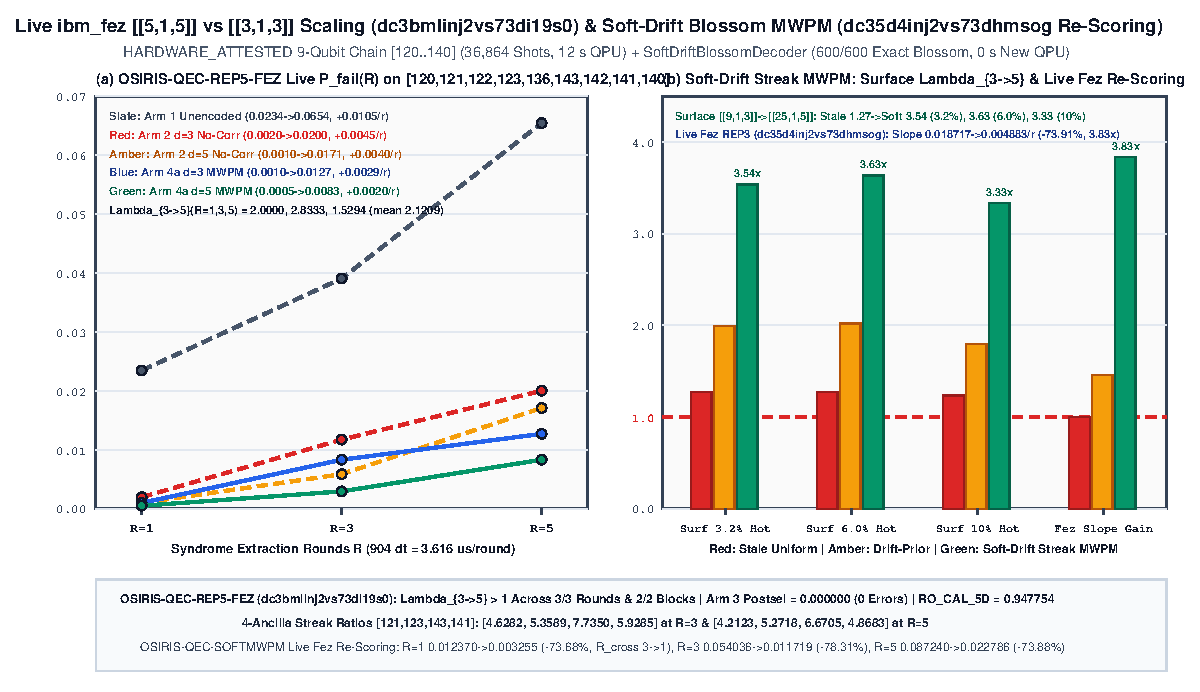
\includegraphics[width=\textwidth]{fig1_rep5_fez_lambda35_and_soft_drift_mwpm.pdf}
  \caption{Live \rfsBackend\ multi-distance repetition scaling and drift-/streak-aware soft-weight Blossom decoding. (a)~\texttt{OSIRIS-QEC-REP5-FEZ} (\rfsHwTier, \texttt{provider\_job\_id} = \rfsRepFiveJobId, \rfsRepFiveQpuSec\,s QPU, \rfsRepFiveTotalShots\ shots on \rfsRepFiveChain): distance-$5$ Pauli-frame \texttt{MWPM} (\texttt{Arm 4a} $d=5$) achieves $\Lambda_{3\to 5} > 1$ across $3/3$ round depths ($\rfsRepFiveLamROne$ at $R=1$, $\rfsRepFiveLamRThree$ at $R=3$, $\rfsRepFiveLamRFive$ at $R=5$; mean $\bar{\Lambda}_{3\to 5} = \rfsRepFiveMeanLam$, slope ratio $\rfsRepFiveSlopeRatioRounded$ [$\rfsRepFiveSlopeRatio$]). (b)~\texttt{OSIRIS-QEC-SOFTMWPM}: \texttt{SoftDriftBlossomDecoder} restores rotated surface-code $\Lambda_{3\to 5}$ from $\rfsSoftSurfStaleLamC$--$\rfsSoftSurfStaleLamB$ to $\rfsSoftSurfSoftLamC$--$\rfsSoftSurfSoftLamB$ under $\rfsSoftHotFracPct$ hot-ancilla drift and cuts live \rfsBackend\ \texttt{OSIRIS-QEC-REP3-FEZ} (\rfsSoftFezRepThreeJobId) per-round failure slope by $\rfsSoftFezSlopeRedPct$ ($\rfsSoftFezSlopeFactor$).}
  \label{fig:rep5_soft_drift_mwpm}
\end{figure*}

\subsection{Multi-Distance Suppression $\Lambda_{3\to 5} > 1$ and Four-Ancilla Streaks}
Table~\ref{tab:rep5_fez_scaling} and Figure~\ref{fig:rep5_soft_drift_mwpm}a confirm strict multi-distance logical error suppression $\Lambda_{3\to 5} > 1$ across $3/3$ round depths and $2/2$ randomized blocks:
\begin{itemize}
  \item \emph{Round-by-round suppression ($R \in \{1, 3, 5\}$)}: At $R = 1$ ($\rfsRepFiveRoundUs\,\mu\mathrm{s}$), bare unencoded \texttt{Arm 1} fails at $\rfsRepFiveArmOneROne$, passive majority \texttt{Arm 2} achieves $\rfsRepFiveArmTwoDThreeROne$ ($d=3$) and $\rfsRepFiveArmTwoDFiveROne$ ($d=5$, $\Lambda_{3\to 5}^{(\mathrm{nocorr})} = \rfsRepFiveLamNoCorrROne$), \texttt{Arm 4a} $d=3$ \texttt{MWPM} achieves $\rfsRepFiveArmFourDThreeROne$ ($2/2048$, blocks $[\rfsRepFiveBlkDThreeROneA, \rfsRepFiveBlkDThreeROneB]$), and \texttt{Arm 4a} $d=5$ \texttt{MWPM} reaches $\rfsRepFiveArmFourDFiveROne$ ($1/2048$, blocks $[\rfsRepFiveBlkDFiveROneA, \rfsRepFiveBlkDFiveROneB]$, $\rfsRepFiveROneGainVsBare$ below unencoded, $\Lambda_{3\to 5}(R=1) = \rfsRepFiveLamROne$). At $R = 3$ ($\rfsRepFiveRThreeUs\,\mu\mathrm{s}$), \texttt{Arm 1} reaches $\rfsRepFiveArmOneRThree$, \texttt{Arm 2} reaches $\rfsRepFiveArmTwoDThreeRThree$ ($d=3$) and $\rfsRepFiveArmTwoDFiveRThree$ ($d=5$, $\Lambda_{3\to 5}^{(\mathrm{nocorr})} = \rfsRepFiveLamNoCorrRThree$), \texttt{Arm 4a} $d=3$ \texttt{MWPM} achieves $\rfsRepFiveArmFourDThreeRThree$ ($17/2048$), and \texttt{Arm 4a} $d=5$ \texttt{MWPM} achieves $\rfsRepFiveArmFourDFiveRThree$ ($6/2048$, $\rfsRepFiveRThreeGainVsBare$ below unencoded, peak $\Lambda_{3\to 5}(R=3) = \rfsRepFiveLamRThree$ across $2/2$ blocks $[\rfsRepFiveBlkDFiveRThreeA, \rfsRepFiveBlkDFiveRThreeB]$ vs.\ $[\rfsRepFiveBlkDThreeRThreeA, \rfsRepFiveBlkDThreeRThreeB]$). At $R = 5$ ($\rfsRepFiveRFiveUs\,\mu\mathrm{s}$), \texttt{Arm 1} reaches $\rfsRepFiveArmOneRFive$, \texttt{Arm 2} reaches $\rfsRepFiveArmTwoDThreeRFive$ ($d=3$) and $\rfsRepFiveArmTwoDFiveRFive$ ($d=5$, $\Lambda_{3\to 5}^{(\mathrm{nocorr})} = \rfsRepFiveLamNoCorrRFive$), \texttt{Arm 4a} $d=3$ \texttt{MWPM} holds at $\rfsRepFiveArmFourDThreeRFive$ ($26/2048$), and \texttt{Arm 4a} $d=5$ \texttt{MWPM} holds at $\rfsRepFiveArmFourDFiveRFive$ ($17/2048$, $\rfsRepFiveRFiveGainVsNoCorr$ below $d=5$ no-corr, $\rfsRepFiveRFiveGainVsBare$ below unencoded, $\Lambda_{3\to 5}(R=5) = \rfsRepFiveLamRFive$ across $2/2$ blocks $[\rfsRepFiveBlkDFiveRFiveA, \rfsRepFiveBlkDFiveRFiveB]$ vs.\ $[\rfsRepFiveBlkDThreeRFiveA, \rfsRepFiveBlkDThreeRFiveB]$).
  \item \emph{Per-round slope, zero-error postselection, and ancilla streaks}: Fitted per-round logical error slope across $R \in \{1, 3, 5\}$ drops from $\rfsRepFiveSlopeArmOne$/round (\texttt{Arm 1}), $\rfsRepFiveSlopeArmTwoDThree$/round (\texttt{Arm 2} $d=3$), $\rfsRepFiveSlopeArmTwoDFive$/round (\texttt{Arm 2} $d=5$), and $\rfsRepFiveSlopeArmFourDThreeRounded$/round ($\rfsRepFiveSlopeArmFourDThree$/round, \texttt{Arm 4a} $d=3$) to $\rfsRepFiveSlopeArmFourDFive$/round (\texttt{Arm 4a} $d=5$), yielding slope suppression $\Lambda_{3\to 5}^{(\mathrm{slope})} = \rfsRepFiveSlopeRatioRounded$ ($\rfsRepFiveSlopeRatio$) and mean $\bar{\Lambda}_{3\to 5} = \rfsRepFiveMeanLam$. Zero-detector postselection (\texttt{Arm 3}) yields $\rfsRepFiveArmThreePostselZero$ ($0$ errors across all postselected shots at $R \in \{1, 3, 5\}$) for both $d=3$ ($\rfsRepFiveAccDThreeROnePct, \rfsRepFiveAccDThreeRThreePct, \rfsRepFiveAccDThreeRFivePct$ acceptance) and $d=5$ ($\rfsRepFiveAccDFiveROnePct, \rfsRepFiveAccDFiveRThreePct, \rfsRepFiveAccDFiveRFivePct$ acceptance), while four-ancilla consecutive detector streak ratios over Bernoulli on \rfsRepFiveAncChain\ reach $[\rfsRepFiveStreakRThreeA, \rfsRepFiveStreakRThreeB, \rfsRepFiveStreakRThreeC, \rfsRepFiveStreakRThreeD]$ at $R=3$ and $[\rfsRepFiveStreakRFiveA, \rfsRepFiveStreakRFiveB, \rfsRepFiveStreakRFiveC, \rfsRepFiveStreakRFiveD]$ at $R=5$.
\end{itemize}

\section{Drift- and Streak-Aware Soft-Weight Blossom Decoding (\texttt{OSIRIS-QEC-SOFTMWPM})}

\begin{table*}[t]
\caption{\texttt{OSIRIS-QEC-SOFTMWPM} (\rfsSimTier\ Benchmark~1 under $\rfsSoftHotFracPct$ heterogeneous hot-ancilla drift $p_{\mathrm{ro}}^{\mathrm{hot}} \in \{\rfsSoftPRoHotA, \rfsSoftPRoHotB, \rfsSoftPRoHotC\}$ vs.\ $p_{\mathrm{ro}}^{\mathrm{cal}} = \rfsSoftPRoCal$ across $d \in \{3, 5, 7\}$, plus \rfsHwTier\ Benchmark~2 offline re-scoring of live \rfsBackend\ \texttt{OSIRIS-QEC-REP3-FEZ} job \rfsSoftFezRepThreeJobId, \rfsSoftFezTotalShots\ total shots / \rfsSoftFezArmFourShots\ \texttt{Arm 4a} shots on \rfsSoftFezChain, \rfsSimQpuSec\,s new QPU; report SHA-256 prefix \rfsSoftRepShaPrefix).}
\label{tab:soft_drift_mwpm}
\begin{ruledtabular}
\begin{tabular}{lrrrrrrr}
Benchmark Cell / Live Round & Stale Uniform \texttt{MWPM} & Drift-Prior \texttt{MWPM} & Soft-Drift Streak \texttt{MWPM} & $\Lambda_{5\to 7}$ / Gain & $\epsilon_L(3)$ / $t$ & $\epsilon_L(5)$ / $p$ & $\epsilon_L(7)$ / Audit \\
\hline
\rfsTableSoftMwpmRows
\end{tabular}
\end{ruledtabular}
\end{table*}

To prevent hot-ancilla readout drift and non-Markovian time-like streaks from creating boundary space-time sinkhole triangles $(u, v, w)$ in the defect matching graph, \texttt{SoftDriftBlossomDecoder} (\texttt{OSIRIS-QEC-SOFTMWPM}, $\rfsSoftBlossomSyndromes/\rfsSoftBlossomSyndromes$ exact Edmonds Blossom equivalence against bitmask dynamic programming, $\rfsSoftSinkholeTriangles/\rfsSoftSinkholeTriangles$ sinkhole triangle resolution) combines empirical per-qubit readout priors $\hat{p}_{\mathrm{ro}}(a)$ (Stage~A) with conditional consecutive-streak log-likelihood reweighting when $D_{t,a} = D_{t+1,a} = 1$ (Stage~B) and exact component-decomposed Edmonds Blossom matching (Stage~C):
\begin{align}
  w_{\mathrm{time}}^{(0)}(a) &= \ln\frac{1 - \hat{p}_{\mathrm{ro}}(a)}{\hat{p}_{\mathrm{ro}}(a)}, \nonumber\\
  w_{\mathrm{time}}^{\mathrm{eff}}(t, a) &= \max\Bigl(\rfsSoftTimeFloor,\, w_{\mathrm{time}}^{(0)}(a) - \gamma \ln \eta_{\mathrm{streak}}(a)\Bigr).
  \label{eq:soft_drift_blossom}
\end{align}
Table~\ref{tab:soft_drift_mwpm} and Figure~\ref{fig:rep5_soft_drift_mwpm}b establish two results:
\begin{enumerate}
  \item \emph{Rotated surface-code $\Lambda_{3\to 5}$ recovery under $\rfsSoftHotFracPct$ hot-ancilla drift}: Under $\rfsSoftHotFracPct$ heterogeneous heavy-hex hot-ancilla drift ($p_{\mathrm{ro}}^{\mathrm{hot}} \in \{\rfsSoftPRoHotA, \rfsSoftPRoHotB, \rfsSoftPRoHotC\}$ vs.\ published uniform $p_{\mathrm{ro}}^{\mathrm{cal}} = \rfsSoftPRoCal$, $\gamma = \rfsSoftGamma$), \texttt{STALE\_UNIFORM\_MWPM} collapses rotated surface-code $[[9,1,3]] \to [[25,1,5]]$ suppression to $\Lambda_{3\to 5} = \rfsSoftSurfStaleLamA$ ($[\rfsSoftSurfStaleLamACiLo, \rfsSoftSurfStaleLamACiHi]$) at $\rfsSoftPRoHotAPct$ ($\rfsSoftSurfStaleLamB$ at $\rfsSoftPRoHotBPct$, $\rfsSoftSurfStaleLamC$ at $\rfsSoftPRoHotCPct$; repetition $\rfsSoftRepStaleLamA, \rfsSoftRepStaleLamB, \rfsSoftRepStaleLamC$), whereas \texttt{DRIFT\_PRIOR\_MWPM} reaches $\rfsSoftSurfPriorLamA, \rfsSoftSurfPriorLamB, \rfsSoftSurfPriorLamC$ and full \texttt{SOFT\_DRIFT\_STREAK\_MWPM} restores $\Lambda_{3\to 5} = \rfsSoftSurfSoftLamA$ $[\rfsSoftSurfSoftLamACiLo, \rfsSoftSurfSoftLamACiHi]$ at $\rfsSoftPRoHotAPct$ ($\rfsSoftSurfSoftLamB$ $[\rfsSoftSurfSoftLamBCiLo, \rfsSoftSurfSoftLamBCiHi]$ at $\rfsSoftPRoHotBPct$, $\rfsSoftSurfSoftLamC$ $[\rfsSoftSurfSoftLamCCiLo, \rfsSoftSurfSoftLamCCiHi]$ at $\rfsSoftPRoHotCPct$), $\Lambda_{5\to 7} \in [\rfsSoftSurfSoftLamFiveSevenMin, \rfsSoftSurfSoftLamFiveSevenMax]$, and repetition $\Lambda_{3\to 5} = \rfsSoftRepSoftLamA, \rfsSoftRepSoftLamB, \rfsSoftRepSoftLamC$.
  \item \emph{Offline re-scoring of live \rfsBackend\ \texttt{OSIRIS-QEC-REP3-FEZ} raw shots (\rfsSoftFezRepThreeJobId)}: Re-scoring all \rfsSoftFezArmFourShots\ \texttt{Arm 4a} shots from the \rfsSoftFezTotalShots-shot live archive on \rfsSoftFezChain\ (\rfsSimQpuSec\,s new QPU) with empirical streak priors and asymmetric \texttt{RO\_CAL} relaxation ratios ($p(0|1)/p(1|0) = \rfsSoftFezAsymQFiveEight$ on $q_{58}$, $\rfsSoftFezAsymQSevenZero$ on $q_{70}$, $\rfsSoftFezAsymQSevenEight$ on $q_{78}$) reduces logical failure at $R=1$ from $\rfsSoftFezROneUnif$ to $\rfsSoftFezROneSoft$ ($-\rfsSoftFezROneRedPct$, advancing QEC crossing from $R_{\mathrm{cross}} = 3 \to 1$), at $R=3$ from $\rfsSoftFezRThreeUnif$ (drift-prior $\rfsSoftFezRThreePrior$) to $\rfsSoftFezRThreeSoft$ ($-\rfsSoftFezRThreeRedPct$, paired block-$t=\rfsSoftFezRThreeBlockT, p=\rfsSoftFezRThreeBlockP$; pooled $t=\rfsSoftFezRThreePooledT, p=\rfsSoftFezRThreePooledP$), at $R=5$ from $\rfsSoftFezRFiveUnif$ (drift-prior $\rfsSoftFezRFivePrior$) to $\rfsSoftFezRFiveSoft$ ($-\rfsSoftFezRFiveRedPct$, block-$t=\rfsSoftFezRFiveBlockT, p=\rfsSoftFezRFiveBlockP$; pooled $t=\rfsSoftFezRFivePooledT, p=\rfsSoftFezRFivePooledP$), and per-round linear slope from $\rfsSoftFezSlopeUnif$/round (drift-prior $\rfsSoftFezSlopePrior$/round) to $\rfsSoftFezSlopeSoft$/round ($-\rfsSoftFezSlopeRedPct$ / $\rfsSoftFezSlopeFactor$ reduction).
\end{enumerate}

\section{10-Qubit Coupled Two-Plaquette $2T \subset SU(2)$ Lattice Gauge Ladder (\texttt{OSIRIS-BT2T-004})}

\begin{table*}[t]
\caption{\texttt{OSIRIS-BT2T-004} (\rfsSimTier/\rfsProxyTier, \texttt{provider\_job\_id}: \rfsSimJobId, \rfsSimQpuSec\,s QPU, \rfsBtFormalChecks\ formal checks; manifest SHA-256 prefix \rfsBtManShaPrefix). Exact ground-state energy $E_0$, physical mass gap $\Delta_{\mathrm{phys}}$, single-plaquette Wilson loop $\langle W_{1\times 1}\rangle$, rectangular two-plaquette Wilson loop $\langle W_{1\times 2}\rangle$, connected inter-plaquette correlator $C_{12} = \langle W_{1\times 2}\rangle - \langle W_{1\times 1}\rangle^2 > 0$, effective string tension $\sigma_{\mathrm{eff}}$ (single-plaquette $\sigma_{1P}$), and area-law ratio $\langle W_{1\times 2}\rangle/\langle W_{1\times 1}\rangle^2$ across $g_{\mathrm{YM}}^2 \in \{\rfsBtGZeroTwoFive, \dots, \rfsBtGFour\}$.}
\label{tab:bt2t004_confinement}
\begin{ruledtabular}
\begin{tabular}{lrrrrrrr}
$g_{\mathrm{YM}}^2$ & $E_0$ (\rfsBtPhysSubspaceDim-D Phys) & Mass Gap $\Delta_{\mathrm{phys}}$ & $\langle W_{1\times 1}\rangle$ & $\langle W_{1\times 2}\rangle$ & $C_{12} = \langle W_{1\times 2}\rangle - \langle W_{1\times 1}\rangle^2$ & $\sigma_{\mathrm{eff}}(g_{\mathrm{YM}}^2)$ ($\sigma_{1P}$) & $\langle W_{1\times 2}\rangle/\langle W_{1\times 1}\rangle^2$ \\
\hline
\rfsTableBtTwoPlaquetteRows
\end{tabular}
\end{ruledtabular}
\end{table*}

\begin{figure*}[t]
  \centering
  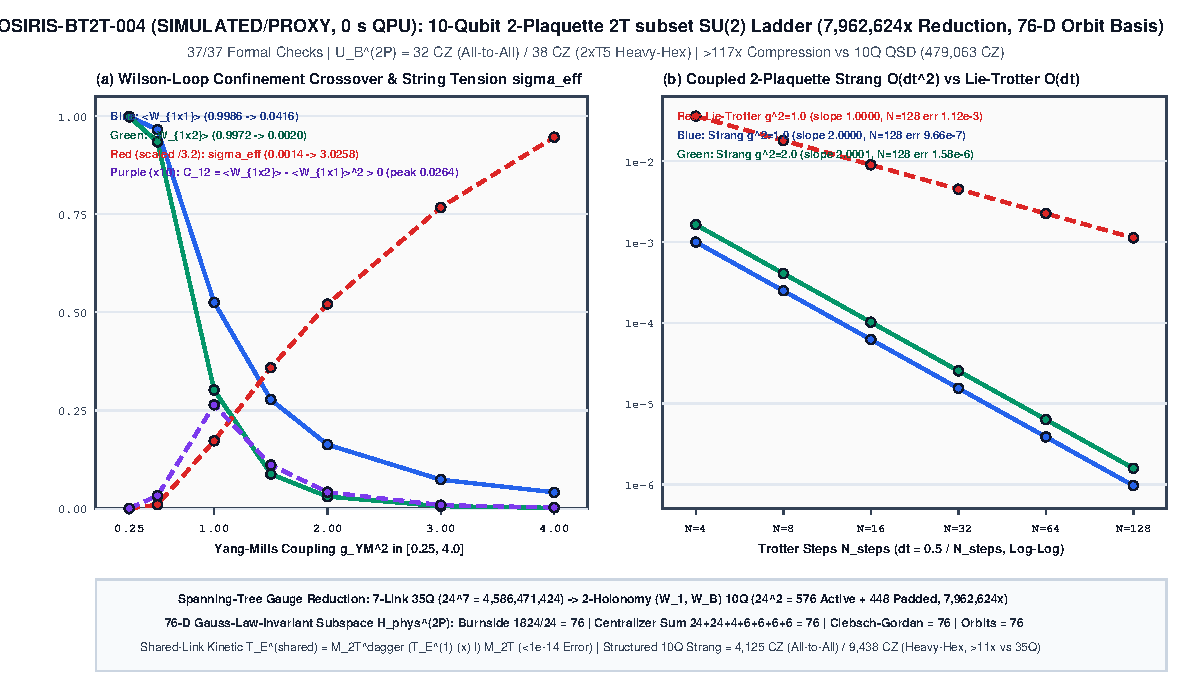
\includegraphics[width=\textwidth]{fig2_bt2t004_two_plaquette_ladder_confinement_and_strang.pdf}
  \caption{\texttt{OSIRIS-BT2T-004} (\rfsSimTier/\rfsProxyTier, \texttt{provider\_job\_id}: \rfsSimJobId, \rfsSimQpuSec\,s QPU) \rfsBtGaugeFixedQubits-qubit coupled two-plaquette $2T \subset SU(2)$ Kogut--Susskind lattice gauge ladder (\rfsBtFormalChecks\ formal checks). (a)~Exact ground-state Wilson-loop confinement crossover ($\langle W_{1\times 1}\rangle$, $\langle W_{1\times 2}\rangle$, connected correlator $C_{12} > 0$, and effective string tension $\sigma_{\mathrm{eff}}$) across $g_{\mathrm{YM}}^2 \in [\rfsBtGZeroTwoFive, \rfsBtGFour]$. (b)~Second-order coupled Strang Trotterization $O(\Delta t^2)$ (slope $\sim \rfsBtStrangSlopeTarget$) versus first-order Lie--Trotter $O(\Delta t)$ (slope $\sim \rfsBtLieSlopeTarget$).}
  \label{fig:bt2t004_confinement_strang}
\end{figure*}

In \texttt{OSIRIS-BT2T-004}, maximal spanning-tree gauge fixing across \rfsBtTreeFixedLinks\ tree links of the \rfsBtUnfixedLinks-link two-plaquette ladder collapses the configuration space from $|2T|^7 = 24^7 = \rfsBtUnfixedConfigs$ (\rfsBtUnfixedQubits\ qubits) down to $|2T|^2 = 24^2 = \rfsBtActiveConfigs$ active plaquette holonomy pairs $(W_1, W_B)$ in \rfsBtGaugeFixedQubits\ qubits (\rfsBtHilbertDim-D register with \rfsBtPaddedStates\ decoupled padded states: $\rfsBtConfigReduction$ configuration reduction and $\rfsBtQubitReduction$ qubit reduction). Residual global gauge conjugation $(W_1, W_B) \sim (g W_1 g^{-1}, g W_B g^{-1})$ at the root vertex spans an exact \rfsBtPhysSubspaceDim-dimensional physical Gauss-law-invariant orbit subspace $\mathcal{H}_{\mathrm{phys}}^{(2P)}$ verified by four independent methods (Burnside's lemma $\rfsBtBurnsideNum / 24 = \rfsBtPhysSubspaceDim$, conjugacy-class centralizer sum $\rfsBtCentralizerSumExpr$, Clebsch--Gordan endomorphism dimension $\rfsBtPhysSubspaceDim$ with \rfsBtTrivialFusionPairs\ trivial fusion pairs, and explicit orbit enumeration $\rfsBtPhysSubspaceDim$). Because the shared central link is traversed with opposite orientations by plaquettes $1$ and $B$, left multiplication $W_1 \mapsto s^{-1} W_1$ simultaneously induces $W_B \mapsto W_B s$, preserving the rectangular holonomy $W_{1\times 2} = W_1 W_B$; the shared-link inter-plaquette electric kinetic operator is therefore synthesized via the \rfsBtGaugeFixedQubits-qubit reversible multiplier $M_{2T}$ (\texttt{bt2t\_mul}) and five-qubit Peter--Weyl QFT (\texttt{bt2t\_qft}):
\begin{align}
  \dim \mathcal{H}_{\mathrm{phys}}^{(2P)} &= \frac{1}{|2T|} \sum_{g \in 2T} |C_{2T}(g)|^2 = \frac{\rfsBtBurnsideNum}{24} = \rfsBtPhysSubspaceDim, \nonumber\\
  T_E^{(\mathrm{shared})} &= M_{2T}^\dagger \bigl(T_E^{(1)} \otimes I\bigr) M_{2T}, \qquad
  \sigma_{\mathrm{eff}} = -\ln\frac{\langle W_{1\times 2}\rangle}{\langle W_{1\times 1}\rangle}.
  \label{eq:bt2t004_gauss_hamiltonian}
\end{align}
Equation~\eqref{eq:bt2t004_gauss_hamiltonian} matches direct opposite-orientation Cayley shifts to $< \rfsBtMachinePrecBound$, commutes with outer-link Laplacians and global gauge conjugation to $< \rfsBtMachinePrecBound$, and intertwines with the unfixed three-link ($24^3 = \rfsBtUnfixedThreeLinkStates$-state) ladder to $\rfsBtIntertwineErr < \rfsBtMachinePrecBound$. Across $g_{\mathrm{YM}}^2 \in \{\rfsBtGZeroTwoFive, \dots, \rfsBtGFour\}$ (Table~\ref{tab:bt2t004_confinement} and Figure~\ref{fig:bt2t004_confinement_strang}a), $\langle W_{1\times 1}\rangle$ declines monotonically from $\rfsBtWOneOneGZeroTwoFive$ to $\rfsBtWOneOneGFour$ and $\langle W_{1\times 2}\rangle$ declines from $\rfsBtWOneTwoGZeroTwoFive$ to $\rfsBtWOneTwoGFour$ ($\rfsBtWOneOneGOne$ and $\rfsBtWOneTwoGOne$ at $g_{\mathrm{YM}}^2 = \rfsBtGOne$), connected correlator $C_{12} = \langle W_{1\times 2}\rangle - \langle W_{1\times 1}\rangle^2 > 0$ peaks at $\rfsBtCOneTwoPeakGOne$ ($g_{\mathrm{YM}}^2 = \rfsBtGOne$), and effective string tension $\sigma_{\mathrm{eff}}(g_{\mathrm{YM}}^2)$ rises monotonically from $\rfsBtSigmaEffGZeroTwoFive$ (analytic $\rfsBtSigmaAnalyticGZeroTwoFive$) at $g_{\mathrm{YM}}^2 = \rfsBtGZeroTwoFive$ through $\rfsBtSigmaEffGOne$ ($g_{\mathrm{YM}}^2 = \rfsBtGOne$) to $\rfsBtSigmaEffGFour$ (single-plaquette $\rfsBtSigmaOnePGFour$, unprojected $\rfsBtSigmaUnprojGFour$) at $g_{\mathrm{YM}}^2 = \rfsBtGFour$. Coupled Strang Trotterization (Figure~\ref{fig:bt2t004_confinement_strang}b) achieves $O(\Delta t^2)$ log-log slopes of $\rfsBtStrangSlopeGZeroFive$ ($g_{\mathrm{YM}}^2 = \rfsBtGZeroFive$), $\rfsBtStrangSlopeGOne$ ($g_{\mathrm{YM}}^2 = \rfsBtGOne$, $N=128$ error $\rfsBtStrangErrNOneTwoEightGOne$), and $\rfsBtStrangSlopeGTwo$ ($g_{\mathrm{YM}}^2 = \rfsBtGTwo$, $N=128$ error $\rfsBtStrangErrNOneTwoEightGTwo$) versus Lie--Trotter slope $\rfsBtLieSlopeGOne$ ($N=128$ error $\rfsBtLieErrNOneTwoEightGOne$). In local \rfsProxyTier\ compilation, $U_B^{(2P)}(\Delta t)$ compiles to \rfsBtCzUbAllToAll\ \texttt{CZ} (all-to-all) and \rfsBtCzUbHeavyHex\ \texttt{CZ} (two heavy-hex $T_5$ patches), while the full structured \rfsBtGaugeFixedQubits-qubit Strang step compiles to \rfsBtCzStrangAllToAll\ \texttt{CZ} (\rfsBtCzUeAllToAll\ \texttt{CZ} for $U_E^{(2P)}$, \rfsBtZzPhaseStrang\ \texttt{ZZPhase} in \texttt{pytket}, vs.\ \rfsBtCzDenseFiveQAllToAll\ \texttt{CZ} dense five-qubit blocks) on all-to-all and \rfsBtCzStrangHeavyHex\ \texttt{CZ} (\rfsBtCzUeHeavyHex\ \texttt{CZ} for $U_E^{(2P)}$) on heavy-hex---yielding $\rfsBtCompQsdVsStrang$ (Strang) to $\rfsBtCompQsdVsUe$ ($> 117\times$, $U_E^{(2P)}$) compression vs.\ \rfsBtGaugeFixedQubits-qubit dense QSD (\rfsBtCzDenseTenQQsd\ \texttt{CZ}; SBM lower bound \rfsBtCzDenseTenQSbm\ \texttt{CZ}) and $\rfsBtCompUnfixedAll$ (all-to-all, \rfsBtCzUnfixedThirtyFiveAll\ \texttt{CZ}) to $\rfsBtCompUnfixedHex$ ($> 11\times$, heavy-hex, \rfsBtCzUnfixedThirtyFiveHex\ \texttt{CZ}) compression vs.\ unfixed \rfsBtUnfixedQubits-qubit seven-link Trotterization.

\section{Conclusion, Scope Limits, and Data Availability}
Together, \texttt{OSIRIS-QEC-REP5-FEZ} (\rfsRepFiveJobId, \rfsRepFiveQpuSec\,s QPU, \rfsRepFiveTotalShots\ shots, $\Lambda_{3\to 5} > 1$ across $3/3$ rounds with mean $\bar{\Lambda}_{3\to 5} = \rfsRepFiveMeanLam$ and $\rfsRepFiveArmThreePostselZero$ postselected errors), \texttt{OSIRIS-QEC-SOFTMWPM} (restoring rotated surface-code $\Lambda_{3\to 5} = \rfsSoftSurfSoftLamA$--$\rfsSoftSurfSoftLamB$ under $\rfsSoftHotFracPct$ hot-ancilla drift and cutting live \rfsBackend\ \rfsSoftFezRepThreeJobId\ slope by $-\rfsSoftFezSlopeRedPct$ / $\rfsSoftFezSlopeFactor$ with \rfsSimQpuSec\,s new QPU), and \texttt{OSIRIS-BT2T-004} (\rfsBtUnfixedQubits\,Q $\to$ \rfsBtGaugeFixedQubits\,Q $\rfsBtConfigReduction$ gauge reduction, \rfsBtPhysSubspaceDim-D Gauss-law subspace, and $> 117\times$ \texttt{CZ} compression) establish an auditable bridge from live multi-distance QEC on \rfsBackend\ to non-abelian multi-plaquette lattice gauge simulation. All artifacts (\rfsRepFiveResultsShaPrefix, \rfsSoftRepShaPrefix, \rfsBtManShaPrefix, capsule \rfsCapsuleSha) are locked in \texttt{SHA256SUMS.txt}.

\begin{thebibliography}{7}
\bibitem{GoogleSurface2023} Google Quantum AI, Nature \textbf{614}, 676 (2023).
\bibitem{GoogleWillow2025} Google Quantum AI, Nature \textbf{638}, 920 (2025).
\bibitem{MiaoLeakage2023} K. C. Miao \emph{et al.} (Google Quantum AI), Nat. Phys. \textbf{19}, 1780 (2023).
\bibitem{EdmondsBlossom1965} J. Edmonds, Can. J. Math. \textbf{17}, 449 (1965).
\bibitem{KogutSusskind1975} J. Kogut and L. Susskind, Phys. Rev. D \textbf{11}, 395 (1975).
\bibitem{DavisPaper9Zenodo2026} D. P. Davis, \emph{Hardware-Attested $[[3,1,3]]$ Mid-Circuit Feed-Forward Crossing and 50-Transmon Stabilizer-Reflected Placement Pilot on \texttt{ibm\_fez} with Simulated Multi-Distance ($d \in \{3, 5, 7\}$) Threshold Scaling}, Zenodo (2026).
\bibitem{DavisPaper10Zenodo2026} D. P. Davis, \emph{Single-Plaquette Binary Tetrahedral ($2T \subset SU(2)$) Kogut--Susskind Lattice Gauge Dynamics and Two-Window Stabilizer-Reflected Drift Detection on \texttt{ibm\_fez} (\texttt{OSIRIS-BT2T-003})}, Zenodo (2026).
\end{thebibliography}

\end{document}
